\section{Actuators}

The actuation system present on the vessel is constituted by the thrusters. These can be divided into two forward thrusters and two side thrusters. 

\subsection{Forward Thrusters}
The forward thrusters are the main actuators present on the vessel and they provide a forward force depending on the rotational speed as 
%
\begin{flalign}
	F(n_\mathrm{PWM}) = \num{0.2567} \cdot n_\mathrm{PWM} - \num{22.83} .
	\label{eq:forwardSpeedForce}
\end{flalign}
%
They can also rotate in the opposite direction, producing a backwards force that can be calculated as 
%
\begin{flalign}
	F(n_\mathrm{PWM}) = \num{0.2567} \cdot n_\mathrm{PWM} - \num{22.83} .
	\label{eq:backwardSpeedForce}
\end{flalign}
%
These equations have been obtained through experimental tests in described in \cite{thesis}.

The forward thrusters are actuated with brushless motors INLINE 750 \num{14.8} V from Graupner. They have two poles with a velocity constant of 1035 rpm kV$^{-1}$ and can operate within \num{7.4} and \num{22.2} V, being the nominal voltage \num{14.8} V. \cite{motors}

\begin{figure}[H]
    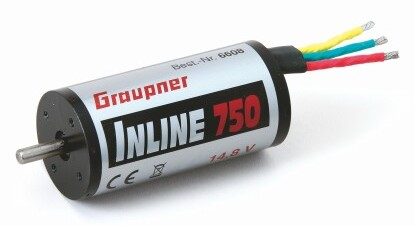
\includegraphics[width=0.4\textwidth]{figures/motor}
    \caption{INLINE 750 \num{14.8} V motor used to produced the forward thrust in the surface vessel \cite{motors}.}
    \label{fig:motors}
\end{figure}

In order to have the motors turning to the desired rotational speed, electronic speed controllers (ESCs) +70 G\num{3,5} from Graupner are used. The operating voltage range goes from 6 to 25 V and they can handle up to 70 A in continuous current. The reference PWM that comes from the microcontroller translates into a 32kHz PWM signal to the speed controller. \cite{ESC}

\begin{figure}[H]
    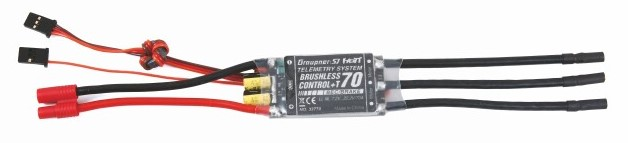
\includegraphics[width=0.8\textwidth]{figures/ESC}
    \caption{Speed controllers +70 G\num{3,5} used to control the forward thrusters in the surface vessel \cite{ESC}.}
    \label{fig:ESC}
\end{figure}

\subsection{Side Thrusters}
The side thrusters move the vessel sideways but their influence in its motion is limited to low speed maneuvers and they are intended for fine positioning of the vessel. For this reason, they are not utilized in the controller design for the vessel.
